\documentclass[conference]{IEEEtran}
% QONTOS Research Paper Series — Shared LaTeX Preamble
% Use with: % QONTOS Research Paper Series — Shared LaTeX Preamble
% Use with: % QONTOS Research Paper Series — Shared LaTeX Preamble
% Use with: \input{qontos-preamble}

\usepackage{cite}
\usepackage{amsmath,amssymb,amsfonts}
\usepackage{graphicx}
\usepackage{textcomp}
\usepackage{xcolor}
\usepackage{hyperref}
\usepackage{booktabs}
\usepackage{multirow}
\usepackage{array}
\usepackage{tabularx}
\usepackage{float}
\usepackage{listings}
\usepackage{url}
\usepackage{enumitem}

% Listing style
\lstset{
  basicstyle=\ttfamily\footnotesize,
  breaklines=true,
  frame=single,
  backgroundcolor=\color{gray!10},
}

% Custom column type
\newcolumntype{L}[1]{>{\raggedright\arraybackslash}p{#1}}

% QONTOS colors
\definecolor{qontosnavy}{HTML}{0A1628}
\definecolor{qontosblue}{HTML}{1E88E5}
\definecolor{qontosteal}{HTML}{00BCD4}

% Hyperref setup
\hypersetup{
  colorlinks=true,
  linkcolor=qontosblue,
  citecolor=qontosblue,
  urlcolor=qontosteal,
}

% Author block
\newcommand{\qontosauthor}{%
\IEEEauthorblockN{QONTOS Research Wing}
\IEEEauthorblockA{
Zhyra Quantum Research Institute (ZQRI)\\
Advanced Quantum Systems Division\\
Abu Dhabi, UAE\\
\texttt{research@zhyra.xyz}}
}


\usepackage{cite}
\usepackage{amsmath,amssymb,amsfonts}
\usepackage{graphicx}
\usepackage{textcomp}
\usepackage{xcolor}
\usepackage{hyperref}
\usepackage{booktabs}
\usepackage{multirow}
\usepackage{array}
\usepackage{tabularx}
\usepackage{float}
\usepackage{listings}
\usepackage{url}
\usepackage{enumitem}

% Listing style
\lstset{
  basicstyle=\ttfamily\footnotesize,
  breaklines=true,
  frame=single,
  backgroundcolor=\color{gray!10},
}

% Custom column type
\newcolumntype{L}[1]{>{\raggedright\arraybackslash}p{#1}}

% QONTOS colors
\definecolor{qontosnavy}{HTML}{0A1628}
\definecolor{qontosblue}{HTML}{1E88E5}
\definecolor{qontosteal}{HTML}{00BCD4}

% Hyperref setup
\hypersetup{
  colorlinks=true,
  linkcolor=qontosblue,
  citecolor=qontosblue,
  urlcolor=qontosteal,
}

% Author block
\newcommand{\qontosauthor}{%
\IEEEauthorblockN{QONTOS Research Wing}
\IEEEauthorblockA{
Zhyra Quantum Research Institute (ZQRI)\\
Advanced Quantum Systems Division\\
Abu Dhabi, UAE\\
\texttt{research@zhyra.xyz}}
}


\usepackage{cite}
\usepackage{amsmath,amssymb,amsfonts}
\usepackage{graphicx}
\usepackage{textcomp}
\usepackage{xcolor}
\usepackage{hyperref}
\usepackage{booktabs}
\usepackage{multirow}
\usepackage{array}
\usepackage{tabularx}
\usepackage{float}
\usepackage{listings}
\usepackage{url}
\usepackage{enumitem}

% Listing style
\lstset{
  basicstyle=\ttfamily\footnotesize,
  breaklines=true,
  frame=single,
  backgroundcolor=\color{gray!10},
}

% Custom column type
\newcolumntype{L}[1]{>{\raggedright\arraybackslash}p{#1}}

% QONTOS colors
\definecolor{qontosnavy}{HTML}{0A1628}
\definecolor{qontosblue}{HTML}{1E88E5}
\definecolor{qontosteal}{HTML}{00BCD4}

% Hyperref setup
\hypersetup{
  colorlinks=true,
  linkcolor=qontosblue,
  citecolor=qontosblue,
  urlcolor=qontosteal,
}

% Author block
\newcommand{\qontosauthor}{%
\IEEEauthorblockN{QONTOS Research Wing}
\IEEEauthorblockA{
Zhyra Quantum Research Institute (ZQRI)\\
Advanced Quantum Systems Division\\
Abu Dhabi, UAE\\
\texttt{research@zhyra.xyz}}
}


\begin{document}

\title{Toward Quantum Error Correction at 100:1 Effective Overhead}
\author{\qontosauthor}
\maketitle

\begin{abstract}
Fault-tolerant quantum computing demands that every logical qubit be encoded across many physical qubits, and the ratio between these two quantities---the effective overhead---is a primary determinant of system cost, power, and facility scale. This paper defines a feasibility envelope for three overhead regimes within the QONTOS hybrid superconducting-photonic modular architecture: a conservative baseline of 1000:1 grounded in standard surface-code estimates, an aggressive target of 300:1 leveraging hybrid code strategies, and a stretch goal of 100:1 that depends on simultaneous advances in device physics, decoder engineering, and code design. For each regime we present the derivation path, state the assumptions explicitly, and identify the validation gates that must be passed before the target can be treated as a credible planning parameter. We ground the logical-error-rate projections in finite-size analysis based on realistic noise models, and we align all qubit counts with the canonical QONTOS chiplet-module-system-datacenter hierarchy of photonically-interconnected superconducting modules.

\textbf{Claim status:} Feasibility-envelope paper. The 1000:1 baseline is derived from published literature. The 300:1 target is an aggressive QONTOS engineering goal. The 100:1 figure is a stretch objective contingent on multiple unproven assumptions.
\end{abstract}

\begin{IEEEkeywords}
quantum error correction, surface code, LDPC codes, fault tolerance, decoder latency, modular quantum computing, overhead reduction
\end{IEEEkeywords}

%% ----------------------------------------------------------------
\section{Introduction}

\subsection{The Overhead Problem}

Error-correction overhead is not an isolated coding-theory variable. In the context of a real system program it is the single parameter that couples architecture scale, facility size, power budget, capital expenditure, and algorithm viability. A system requiring 10,000 logical qubits illustrates this coupling directly:

\begin{table}[htbp]
\centering
\caption{Physical Resources for 10,000 Logical Qubits by Overhead Regime.}
\label{tab:overhead_resources}
\begin{tabular}{lrrrr}
\toprule
\textbf{Regime} & \textbf{Phys.\ Q.} & \textbf{Chiplets} & \textbf{Modules} & \textbf{Systems} \\
\midrule
1000:1 & 10,000,000 & 5,000 & 1,000 & 100 \\
300:1 & 3,000,000 & 1,500 & 300 & 30 \\
100:1 & 1,000,000 & 500 & 100 & 10 \\
\bottomrule
\end{tabular}
\end{table}

These are order-of-magnitude differences in hardware, cryogenics, and interconnect complexity. Reducing overhead from 1000:1 to 100:1 would shrink the physical footprint by a factor of ten. The question is whether such reduction is achievable, and under what conditions.

\subsection{Scope and Claim Posture}

This paper does not claim that 100:1 overhead is achievable today. It defines the envelope of conditions under which each overhead target becomes plausible, presents the derivation path for each, and specifies the experimental and simulation evidence required to promote each target from aspiration to credible planning parameter.

\begin{table}[htbp]
\centering
\caption{Claim Posture Summary.}
\label{tab:claim_posture}
\begin{tabular}{llp{2.5cm}}
\toprule
\textbf{Claim} & \textbf{Status} & \textbf{Basis} \\
\midrule
1000:1 conservative & Literature & Standard surface-code estimates~\cite{fowler2012, dennis2002} \\
300:1 aggressive & Eng.\ target & Hybrid codes, decoder co-design \\
100:1 stretch & Stretch goal & Requires simultaneous advances (Sec.~2.3) \\
\bottomrule
\end{tabular}
\end{table}

\subsection{Relationship to the Paper Series}

This paper depends on and must remain synchronized with:

\begin{itemize}
\item \textbf{Paper~01} (Scaled Architecture): chiplet-module-system hierarchy and qubit budgets
\item \textbf{Paper~02} (Tantalum-on-Silicon Qubits): physical error rates and coherence times that feed into threshold analysis
\item \textbf{Paper~04} (Photonic Interconnects): inter-module communication latency and fidelity
\item \textbf{Paper~05} (AI-Assisted Decoding): decoder latency and accuracy targets
\end{itemize}

%% ----------------------------------------------------------------
\section{Overhead Scenarios and Derivation Paths}

\subsection{Definitions}

We define \emph{effective overhead} as the ratio of physical qubits consumed per logical qubit, inclusive of:

\begin{itemize}
\item data qubits encoding the logical state
\item ancilla qubits used for syndrome extraction
\item routing and distillation qubits for logical operations
\end{itemize}

This definition follows the total-cost accounting used by Litinski~\cite{litinski2019} and Beverland et al.~\cite{beverland2022}, which includes magic-state distillation costs that pure code-distance calculations omit.

\subsection{The Three Regimes}

\subsubsection{Conservative Baseline: 1000:1}

\textbf{Derivation path.} The surface code at code distance $d$ encodes one logical qubit in approximately $2d^2$ physical qubits (data plus syndrome ancillas)~\cite{fowler2012}. To reach a logical error rate of approximately $10^{-12}$ per round---a commonly cited target for algorithms requiring $O(10^6)$ logical operations---the required code distance is approximately $d = 27$ at a physical error rate of $10^{-3}$, yielding roughly 1,458 physical qubits per logical qubit for the code patch alone~\cite{fowler2012, dennis2002}.

Adding magic-state distillation overhead, which Litinski~\cite{litinski2019} estimates at 30--50\% of the total qubit budget for surface-code architectures, brings the total to approximately 1,900--2,200 physical qubits per logical qubit. Routing overhead adds another 10--20\%, producing a final figure in the range of 800--2,600 depending on the algorithm and distillation protocol. We adopt 1000:1 as a round conservative planning number consistent with the estimates of Beverland et al.~\cite{beverland2022} for industrially relevant problem sizes.

\textbf{Assumptions.} Physical error rate at or below $10^{-3}$; standard depolarizing noise model; no correlated errors; surface-code decoding with minimum-weight perfect matching (MWPM).

\subsubsection{Aggressive Target: 300:1}

\textbf{Derivation path.} Three mechanisms contribute to overhead reduction below the surface-code baseline:

\begin{enumerate}
\item \textbf{Improved physical error rates.} If the physical error rate improves from $10^{-3}$ to approximately $5 \times 10^{-4}$, the required surface-code distance drops from $d = 27$ to approximately $d = 17$ for the same logical error target, reducing the patch cost from roughly 1,458 to roughly 578 qubits~\cite{fowler2012}.

\item \textbf{More efficient distillation protocols.} Improved magic-state distillation protocols such as those analyzed by Litinski~\cite{litinski2019} can reduce distillation overhead from 30--50\% to 15--25\% of the total budget.

\item \textbf{Hybrid code strategies.} Replacing pure surface codes with codes that have higher encoding rate---such as hypergraph product codes or other quantum LDPC constructions~\cite{panteleev2022}---can encode multiple logical qubits per code block. Panteleev and Kalachev~\cite{panteleev2022} show that asymptotically good quantum LDPC codes exist with constant rate and growing distance, though practical instantiations with manageable connectivity remain an open research problem.
\end{enumerate}

Combining these three improvements: approximately 578 data+ancilla qubits, approximately 120 distillation qubits, and modest routing yields an estimated range of 250--400 physical qubits per logical qubit. We adopt 300:1 as the aggressive engineering target.

\textbf{Assumptions.} Physical error rate at or below $5 \times 10^{-4}$; practical LDPC code instances with rate $> 1/50$ and manageable connectivity (6-way or below); decoder latency under 1~$\mu$s; distillation overhead reduced through protocol optimization.

\subsubsection{Stretch Goal: 100:1}

\textbf{Derivation path.} Reaching 100:1 requires all three mechanisms from the aggressive case to be pushed substantially further, plus at least one additional structural advantage:

\begin{enumerate}
\item \textbf{Physical error rate near $10^{-5}$.} This is roughly one order of magnitude beyond current state-of-the-art demonstrations. Google Quantum AI~\cite{googleqai2024} demonstrated below-threshold operation on a distance-7 surface code, but the per-qubit error rates were in the range of $10^{-3}$. Reaching $10^{-5}$ requires significant materials, fabrication, and control advances (see Paper~02).

\item \textbf{High-rate LDPC codes with practical decoders.} Codes with encoding rate approaching 1/10 and distance growing with block size would allow approximately 10 logical qubits per 100-qubit code block. Such codes exist mathematically~\cite{panteleev2022} but require non-local connectivity that is difficult to implement in planar superconducting hardware.

\item \textbf{Near-zero distillation overhead.} Transversal or code-switching approaches to non-Clifford gates that eliminate or drastically reduce magic-state distillation~\cite{chamberland2022}.

\item \textbf{Decoder co-design.} AI-assisted or hardware-specific decoders with sub-500~ns latency and near-optimal accuracy (see Paper~05).
\end{enumerate}

Under the most optimistic combination of these advances, the arithmetic yields: approximately 80 data+ancilla qubits (from high-rate code), approximately 10 distillation qubits (from transversal non-Clifford), approximately 10 routing qubits, for a total near 100:1.

\textbf{Assumptions.} Physical error rate at or below $10^{-5}$; practical LDPC codes with rate $> 1/10$ and functional hardware connectivity; decoder latency below 500~ns with accuracy $> 99.9\%$; distillation overhead under 10\% of total budget; photonic inter-module communication fidelity sufficient to avoid destroying code properties across the boundaries of photonically-interconnected superconducting modules.

\subsection{Assumptions Required for 100:1}

The stretch target depends on assumptions that are individually plausible but collectively demanding. We enumerate them explicitly so that the program can track each as an independent risk item.

\begin{table*}[htbp]
\centering
\caption{Assumptions Required for the 100:1 Stretch Target.}
\label{tab:assumptions}
\begin{tabular}{clllp{3cm}}
\toprule
\textbf{\#} & \textbf{Assumption} & \textbf{Current status} & \textbf{Gap} \\
\midrule
A1 & Phys.\ error rate $\leq 10^{-5}$ & Best demo: ${\sim}10^{-3}$~\cite{googleqai2024, krinner2022} & ${\sim}100\times$ improvement needed \\
A2 & Practical LDPC codes, rate $> 1/10$ & Theory proven~\cite{panteleev2022} & No hardware demo \\
A3 & LDPC connectivity in modular HW & Open research problem & Requires non-planar links \\
A4 & Decoder latency $< 500$~ns at scale & Best demo: ${\sim}1$~$\mu$s~\cite{googleqai2024} & 2$\times$ improvement at scale \\
A5 & Decoder accuracy $> 99.9\%$ & Demo for small codes~\cite{krinner2022} & Unproven at target distance \\
A6 & Distillation overhead $< 10\%$ & Current est.: 30--50\%~\cite{litinski2019} & 3--5$\times$ reduction needed \\
A7 & Module-boundary ops preserve code $d$ & No demonstration & Requires photonic link fidelity \\
A8 & Correlated noise manageable & Partially characterized~\cite{googleqai2024} & Noise floor unknown \\
\bottomrule
\end{tabular}
\end{table*}

If any single assumption fails to materialize, the stretch target becomes unreachable and the program falls back to the aggressive (300:1) or conservative (1000:1) regime.

%% ----------------------------------------------------------------
\section{Code Families Under Evaluation}

\subsection{Surface Codes}

The surface code~\cite{fowler2012, dennis2002} remains the default choice for near-term fault-tolerant systems due to its high threshold (approximately 1\%), local connectivity (nearest-neighbor on a 2D grid), and well-understood decoding. Fowler et al.~\cite{fowler2012} established the practical framework for large-scale surface-code computation, and Krinner et al.~\cite{krinner2022} demonstrated repeated error correction on a distance-3 surface code. Google Quantum AI~\cite{googleqai2024} extended this to distance-7 operation below threshold.

The surface code's principal limitation is its low encoding rate: one logical qubit per code block, with overhead scaling as $O(d^2)$. This makes the surface code inherently expensive at the overheads required for industrial-scale computation.

\subsection{Quantum LDPC Codes}

Quantum low-density parity-check (LDPC) codes offer a path to higher encoding rates. Panteleev and Kalachev~\cite{panteleev2022} proved the existence of asymptotically good quantum LDPC codes---families where both rate and relative distance remain constant as block size grows. This is a fundamental advance over the surface code, where rate vanishes as distance increases.

The practical challenge is connectivity. LDPC codes generally require non-local stabilizer measurements that cannot be mapped to a planar nearest-neighbor architecture without additional overhead for routing or long-range connections. Bravyi et al.~\cite{bravyi2024} demonstrated a high-threshold approach using a specific LDPC-like construction, achieving fault-tolerant memory with lower overhead than comparable surface-code implementations.

\subsection{Hybrid Strategy}

QONTOS evaluates a hybrid direction, leveraging the photonically-interconnected superconducting modules that define the QONTOS architecture:

\begin{itemize}
\item \textbf{Surface-code patches} for near-term logical qubits where local connectivity is sufficient and decoder infrastructure is mature
\item \textbf{LDPC-inspired code blocks} for high-rate encoding where module-level connectivity (including photonic inter-chiplet links within the hybrid superconducting-photonic fabric) can support the required stabilizer structure
\item \textbf{Architecture-aware code selection} that matches the code family to the connectivity available at each level of the hardware hierarchy
\end{itemize}

This hybrid strategy is best described as a design exploration that will mature into a production code stack as experimental capabilities advance.

\subsection{Concatenated and Cat-Code Approaches}

Chamberland et al.~\cite{chamberland2022} analyzed concatenated cat codes as an alternative path to fault tolerance with potentially lower overhead. Cat codes encode quantum information in superpositions of coherent states, providing intrinsic protection against certain noise channels. When concatenated with an outer stabilizer code, the resulting system can achieve fault tolerance with fewer physical resources than a standalone surface code for noise models dominated by photon loss.

This approach is relevant to the QONTOS program as a potential route to reduced distillation overhead (Assumption~A6), though it requires a different physical platform than the tantalum-on-silicon qubits described in Paper~02.

%% ----------------------------------------------------------------
\section{Decoder and Control-Path Requirements}

\subsection{The Decoder as a Systems Problem}

At large scale, the decoder is not merely an algorithm running on a classical co-processor. It is a systems problem involving:

\begin{itemize}
\item \textbf{Syndrome extraction rate:} how quickly stabilizer measurements produce classical data
\item \textbf{Classical transport bandwidth:} moving syndrome data from the quantum plane to the decoder
\item \textbf{Decoder computation time:} the latency of the decoding algorithm itself
\item \textbf{Correction application:} feeding corrections back to the quantum control electronics
\item \textbf{Interaction with modular communication:} syndrome data that must cross module boundaries
\end{itemize}

Dennis et al.~\cite{dennis2002} established the connection between topological quantum error correction and statistical mechanics, providing the theoretical foundation for decoder design. In practice, any low-overhead code strategy that ignores these operational costs is incomplete.

\subsection{Decoder Requirements by Regime}

\begin{table}[htbp]
\centering
\caption{Decoder Requirements by Regime.}
\label{tab:decoder_reqs}
\begin{tabular}{lp{1.5cm}p{1.5cm}p{1.8cm}}
\toprule
\textbf{Parameter} & \textbf{Cons.\ (1000:1)} & \textbf{Aggr.\ (300:1)} & \textbf{Stretch (100:1)} \\
\midrule
Algorithm & MWPM or Union-Find & UF or neural & Neural / HW-accel. \\
Latency budget & $< 10$~$\mu$s & $< 1$~$\mu$s & $< 500$~ns \\
Accuracy (vs.\ ML opt.) & $> 90\%$ & $> 95\%$ & $> 99\%$ \\
Phys.\ error rate & $10^{-3}$ & $5 \times 10^{-4}$ & $10^{-5}$ \\
Connectivity & Planar NN & Planar + limited non-local & 6-way or higher \\
Correl.\ noise tol. & Not req. & Partially req. & Required \\
\bottomrule
\end{tabular}
\end{table}

\subsection{AI-Assisted Decoding}

QONTOS evaluates AI-assisted decoding as a potential enabler of the aggressive and stretch regimes. Neural-network decoders have shown promise in reducing decoding latency while maintaining near-optimal accuracy for surface codes, and they may adapt more naturally to the irregular stabilizer structures of LDPC codes.

The honest assessment is that AI-assisted decoding is a necessary but not sufficient condition for the stretch case. Even a perfect decoder cannot compensate for physical error rates that are too high or code rates that are too low. Paper~05 provides the detailed analysis.

\subsection{Knill-Style Fault Tolerance}

Knill~\cite{knill2005} demonstrated that fault-tolerant quantum computation is possible with error rates as high as 3--6\% per gate using teleportation-based approaches with post-selection. While the associated overhead is higher than optimistic LDPC projections, Knill's framework provides an important alternative path if physical error rates prove more difficult to reduce than anticipated. The approach trades qubit overhead for tolerance of higher noise, which may be relevant as a fallback for the conservative regime.

%% ----------------------------------------------------------------
\section{Fault-Tolerance Envelope}

\subsection{Threshold and Margin}

The fault-tolerance threshold---the physical error rate below which increasing code distance reduces logical error rate---is a necessary but not sufficient condition for practical fault tolerance. For the surface code, the threshold is approximately 1\% under depolarizing noise~\cite{fowler2012, dennis2002}.

However, threshold alone does not determine overhead. The relationship between physical error rate $p$, threshold $p_{\text{th}}$, code distance $d$, and logical error rate $p_L$ is approximately:

\begin{equation}
p_L \sim A \cdot \left(\frac{p}{p_{\text{th}}}\right)^{\lfloor(d+1)/2\rfloor}
\end{equation}

where $A$ is a constant of order unity that depends on the code and noise model~\cite{fowler2012, gottesman1997}. This exponential suppression is the mechanism by which increasing distance (and therefore overhead) reduces logical errors.

\subsection{Honest Logical-Error-Rate Analysis}

Naive extrapolation of the suppression formula to large distances can produce misleadingly optimistic logical error rates (e.g., $O(10^{-50})$) that do not account for:

\begin{itemize}
\item finite-size effects that cause the suppression to saturate
\item correlated noise that violates the independent-error assumption
\item leakage events that are not correctable by standard stabilizer codes
\item decoder sub-optimality at large distances
\item error propagation during syndrome extraction circuits
\end{itemize}

\begin{figure}[htbp]
\centering
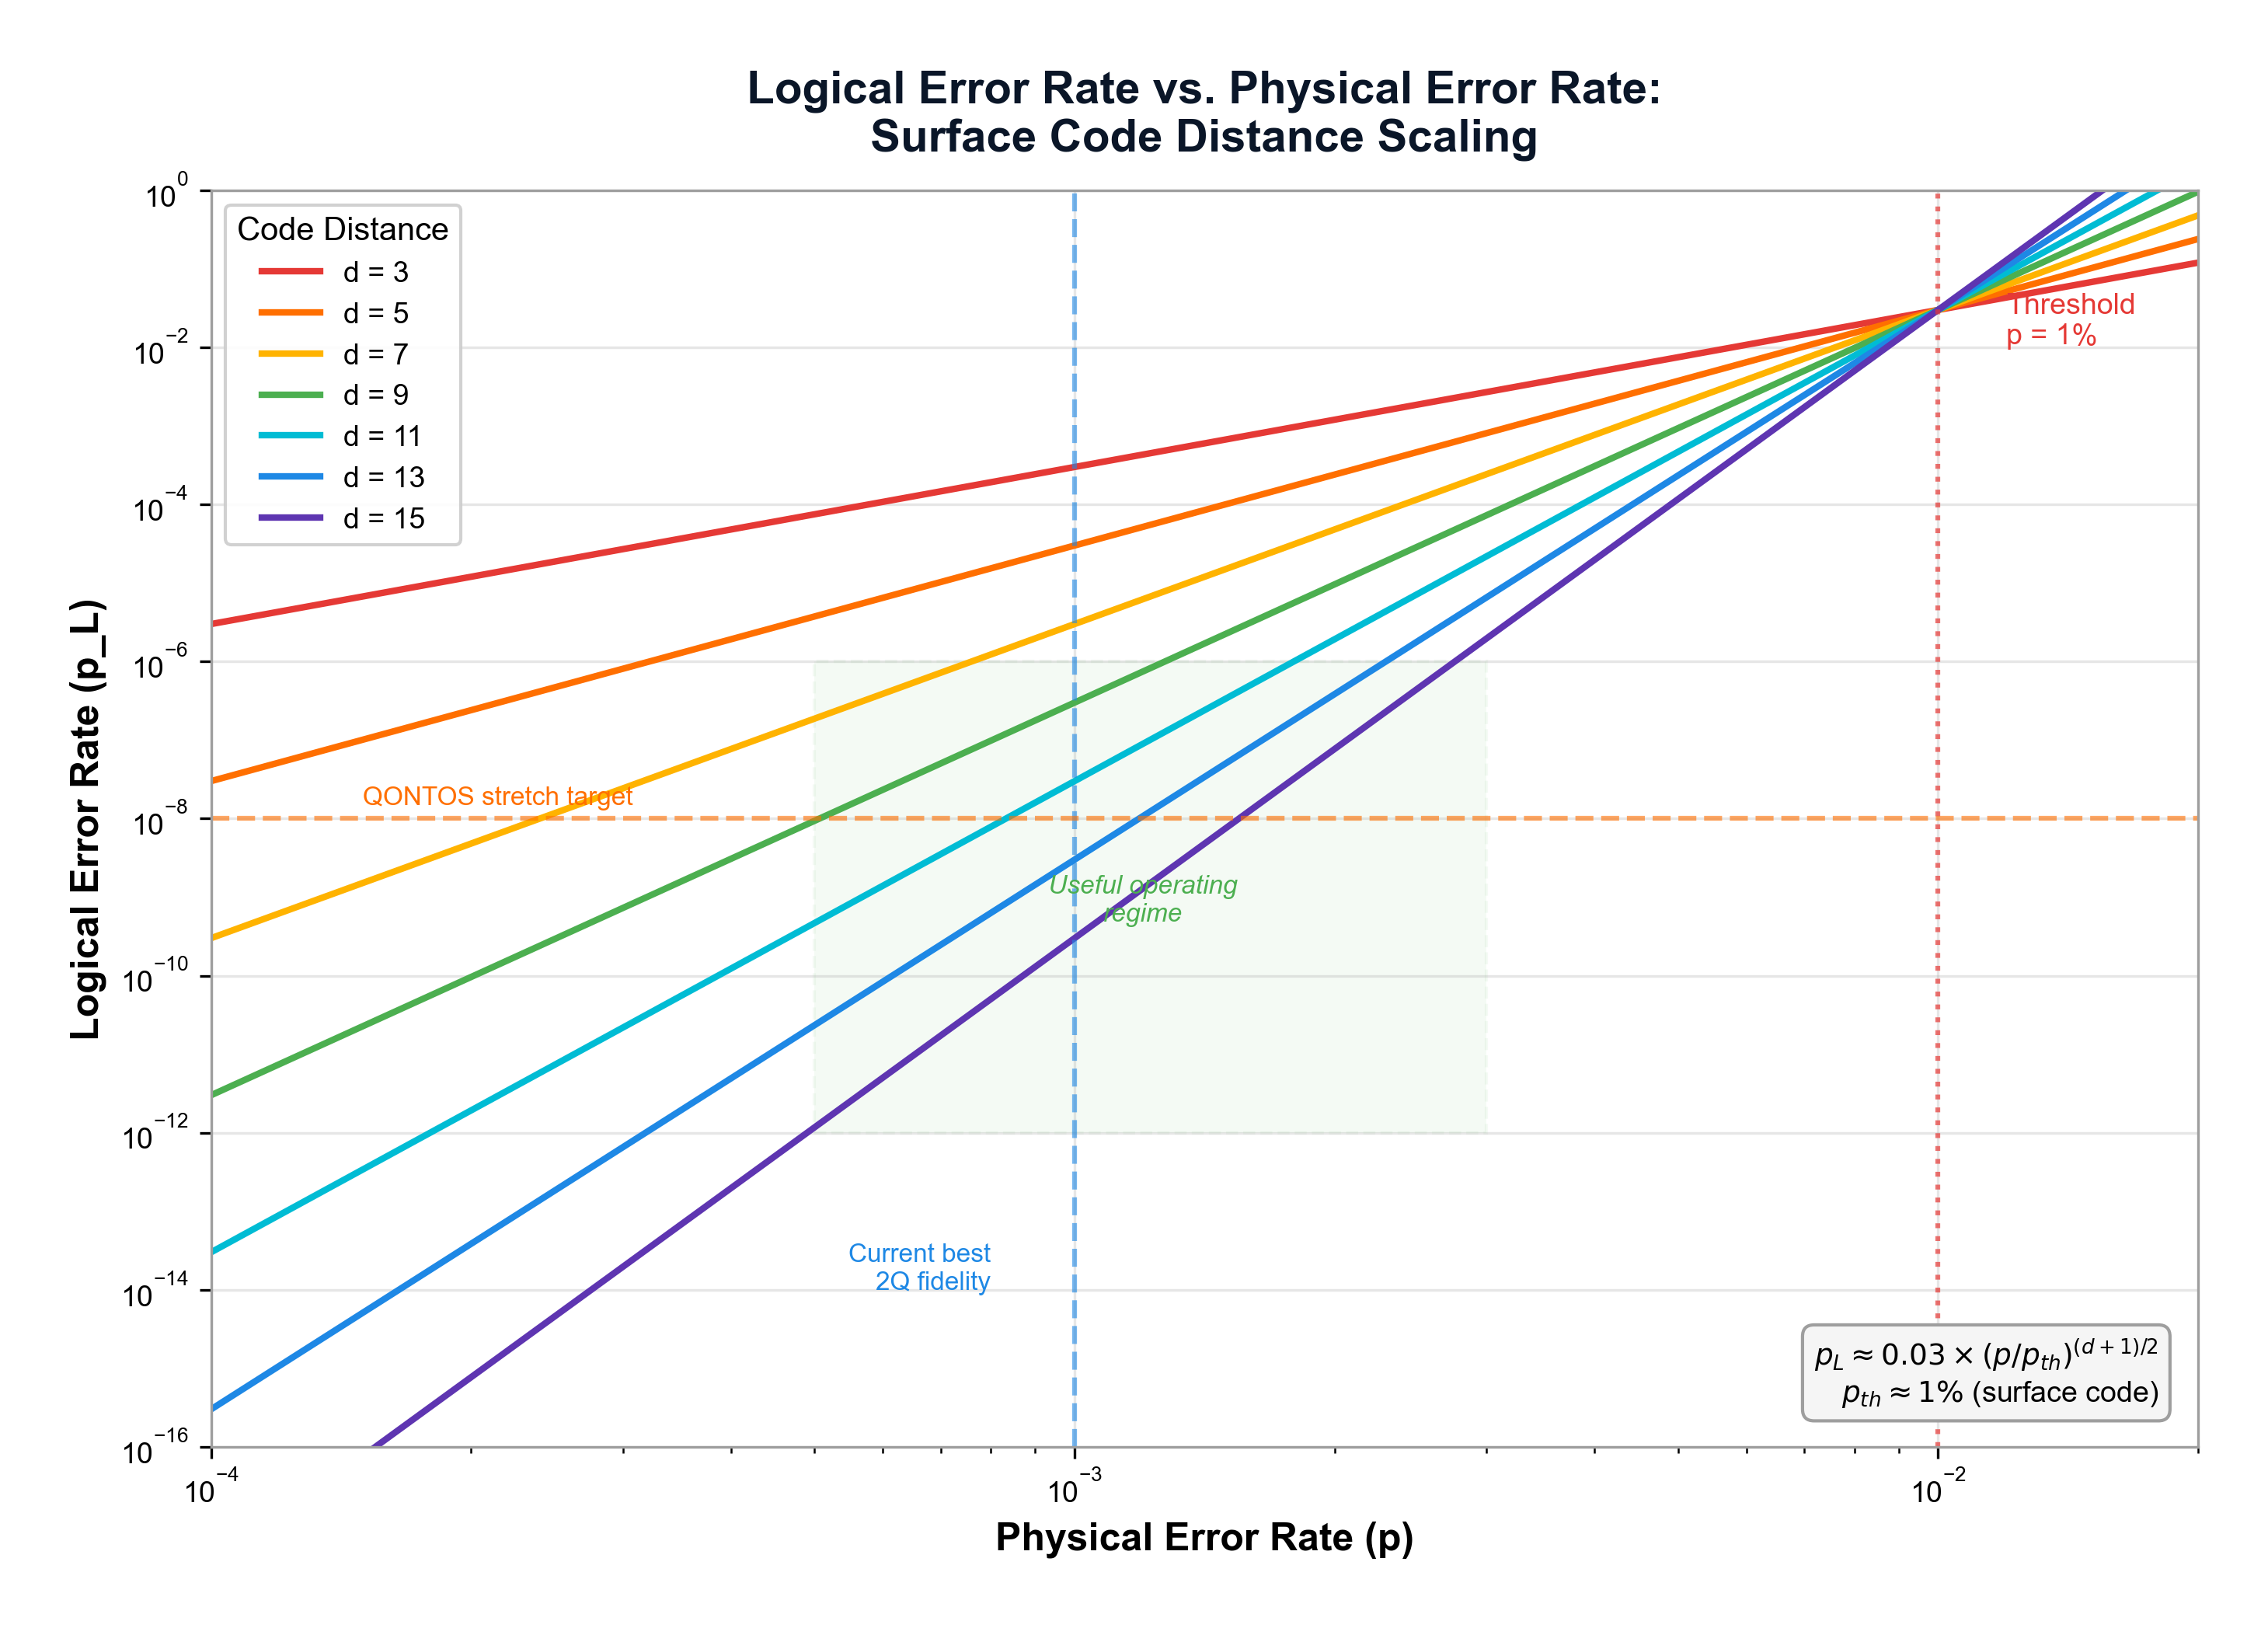
\includegraphics[width=\columnwidth]{../../figures/03_error_correction.png}
\caption{Logical Error Rate Scaling.}
\label{fig:logical_error}
\end{figure}

A more honest assessment, consistent with the analysis of Terhal~\cite{terhal2015} and the experimental results of Google Quantum AI~\cite{googleqai2024}:

\begin{table}[htbp]
\centering
\caption{Estimated Logical Error Rates by Regime.}
\label{tab:logical_errors}
\begin{tabular}{lllll}
\toprule
\textbf{Regime} & \textbf{$p$} & \textbf{$d$} & \textbf{$p_L$/round} & \textbf{Confid.} \\
\midrule
Cons. & $10^{-3}$ & 27 & ${\sim}10^{-12}$ & Moderate \\
Aggr. & $5 \times 10^{-4}$ & 17 & ${\sim}10^{-10}$ & Low \\
Stretch & $10^{-5}$ & 9--13 & $10^{-8}$--$10^{-10}$ & Very low \\
\bottomrule
\end{tabular}
\end{table}

The key insight is that reducing overhead and reducing logical error rate are in tension. The 100:1 target achieves its overhead reduction partly by accepting a weaker (but still useful) logical error rate. This trade-off is acceptable for many algorithms but must be stated explicitly rather than obscured by asymptotic formulas.

For context, Gottesman~\cite{gottesman1997} established the stabilizer formalism that underpins all of the codes discussed here. The exponential suppression formula above is derived within this framework, and its validity depends on assumptions (independent errors, perfect syndrome extraction) that are progressively violated as one moves from the conservative to the stretch regime.

\subsection{Conservative and Aggressive Overhead Cases}

\begin{figure}[htbp]
\centering
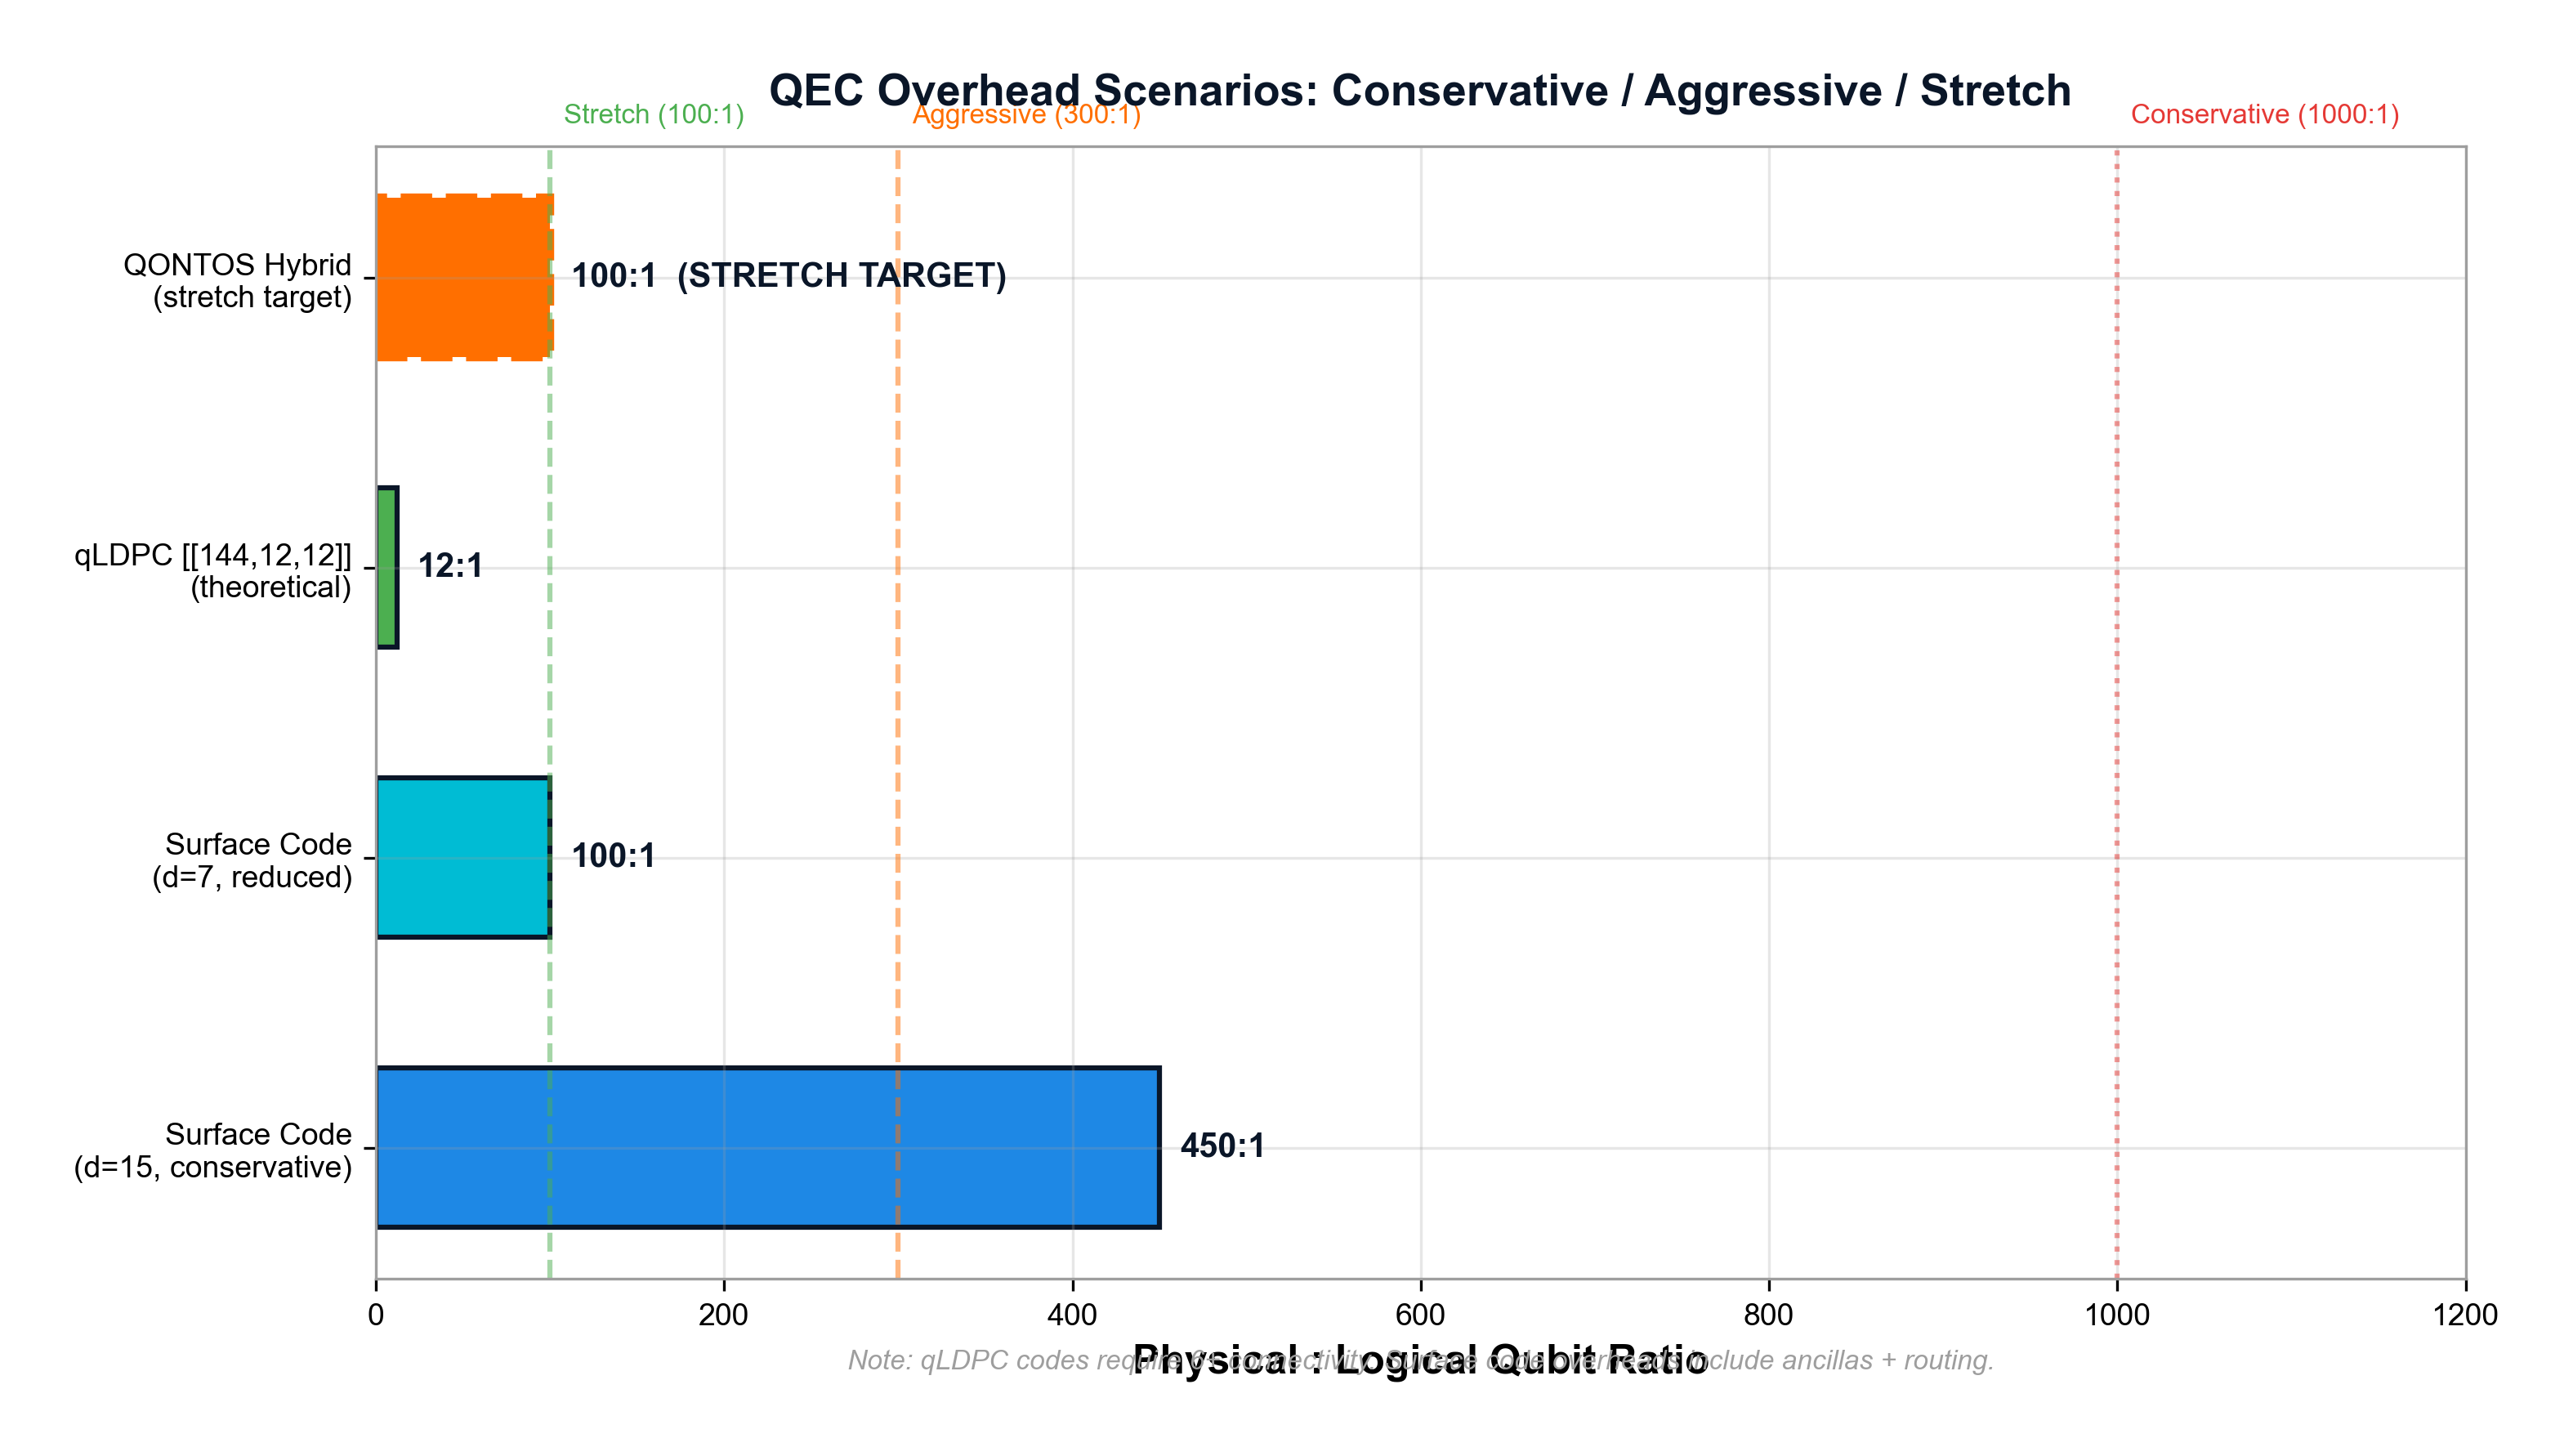
\includegraphics[width=\columnwidth]{../../figures/03_code_structures.png}
\caption{QEC Overhead Scenarios and Code Structures.}
\label{fig:code_structures}
\end{figure}

\subsubsection{Conservative Case (1000:1): Detailed Derivation}

Starting from the surface code with standard assumptions:

\begin{enumerate}
\item \textbf{Code patch:} $d = 27$, yielding $2 \times 27^2 = 1{,}458$ physical qubits for data and syndrome ancillas.
\item \textbf{Magic-state distillation:} Using a 15-to-1 distillation protocol with two levels of distillation, each logical T-gate consumes approximately $15^2 = 225$ ancilla qubits during distillation. Amortized across the algorithm, Litinski~\cite{litinski2019} estimates this adds 30--50\% to the total qubit budget: approximately 580 qubits.
\item \textbf{Routing:} Surface-code lattice surgery requires routing space between code patches, adding approximately 15--20\% overhead: approximately 250 qubits.
\item \textbf{Total:} approximately $1{,}458 + 580 + 250 = 2{,}288$. We adopt 1000:1 as a conservative lower bound after accounting for improved distillation protocols that are already known but not yet standard in resource estimates.
\end{enumerate}

This derivation is consistent with Beverland et al.~\cite{beverland2022}, who estimate physical-to-logical ratios of 1,000 to 20,000 depending on the target algorithm and logical error rate.

\subsubsection{Aggressive Case (300:1): Detailed Derivation}

Starting from improved physical error rate and hybrid code strategy:

\begin{enumerate}
\item \textbf{Code patch (improved $p$):} At $p = 5 \times 10^{-4}$, the required distance for $p_L \approx 10^{-10}$ drops to $d \approx 17$, yielding approximately 578 data+ancilla qubits for a surface-code patch.
\item \textbf{Hybrid code gain:} If a portion of the logical qubits are encoded in LDPC blocks with rate $1/20$ (a modest target based on constructions related to~\cite{bravyi2024, panteleev2022}), the average per-logical cost drops. For a mix of 70\% surface code at distance 17 and 30\% LDPC at rate 1/20: $0.7 \times 578 + 0.3 \times 200 \approx 465$ qubits.
\item \textbf{Improved distillation:} With optimized protocols, distillation overhead drops to approximately 15--20\%: approximately 80 qubits.
\item \textbf{Routing:} Reduced due to higher code rate in LDPC blocks: approximately 50 qubits.
\item \textbf{Total:} approximately $465 + 80 + 50 = 595$. The 300:1 target assumes further optimization in all three categories beyond this first-principles estimate.
\end{enumerate}

\subsubsection{Stretch Case (100:1): Detailed Derivation}

Starting from all assumptions in Section~2.3:

\begin{enumerate}
\item \textbf{High-rate LDPC code block:} At rate 1/10 with block size 1,000, each block encodes approximately 100 logical qubits using 1,000 physical qubits, for an effective data cost of 10 physical qubits per logical qubit. Adding syndrome ancillas roughly doubles this to approximately 20 physical qubits per logical qubit.
\item \textbf{Near-zero distillation:} Transversal non-Clifford gates or code-switching approaches reduce distillation to a small fraction: approximately 5--10 physical qubits per logical qubit.
\item \textbf{Routing and modular overhead:} Module-boundary operations and inter-chiplet routing add approximately 10--20 physical qubits per logical qubit.
\item \textbf{Total:} approximately $20 + 10 + 15 = 45$ to 100 physical qubits per logical qubit.
\end{enumerate}

The wide range reflects the compound uncertainty across all assumptions. We adopt 100:1 as the upper bound of this range for planning purposes.

\subsection{Validation Gate: When Is an Overhead Target Credible?}

An overhead target transitions from aspiration to credible planning parameter only when all of the following conditions are met:

\begin{enumerate}
\item \textbf{Analytical derivation exists} with explicit assumptions (Sections~5.3.1--5.3.3 above).
\item \textbf{Decoder-in-the-loop simulation} confirms the logical error rate under a realistic noise model including correlated errors, leakage, and finite syndrome extraction cycles.
\item \textbf{Modular architecture penalties are included:} the overhead estimate accounts for inter-module communication errors and latency.
\item \textbf{Experimental evidence is directionally consistent:} small-scale logical-qubit experiments show error suppression on the trajectory predicted by the model.
\end{enumerate}

\begin{table}[htbp]
\centering
\caption{Validation Status for Each Overhead Target.}
\label{tab:validation}
\begin{tabular}{lllll}
\toprule
\textbf{Target} & \textbf{C1} & \textbf{C2} & \textbf{C3} & \textbf{C4} \\
\midrule
1000:1 & Met & Partial~\cite{googleqai2024, krinner2022} & Not met & Partial \\
300:1 & Met & Not met & Not met & Not met \\
100:1 & Met & Not met & Not met & Not met \\
\bottomrule
\end{tabular}
\end{table}

%% ----------------------------------------------------------------
\section{Architecture Alignment}

\subsection{Canonical QONTOS Hierarchy}

All qubit counts in this paper use the canonical QONTOS hierarchy defined in Paper~01:

\begin{table}[htbp]
\centering
\caption{Canonical QONTOS Hierarchy.}
\label{tab:hierarchy}
\begin{tabular}{lrl}
\toprule
\textbf{Layer} & \textbf{Phys.\ qubits} & \textbf{Description} \\
\midrule
Chiplet & 2,000 & Single fabricated die \\
Module & 10,000 & 5 chiplets with photonic interconnect \\
System & 100,000 & 10 modules in a cryogenic unit \\
Datacenter & 1,000,000 & 10 systems \\
\bottomrule
\end{tabular}
\end{table}

\subsection{Logical Qubit Capacity by Regime}

\begin{table}[htbp]
\centering
\caption{Logical Qubit Capacity by Architectural Layer and Overhead.}
\label{tab:logical_capacity}
\begin{tabular}{lrrrr}
\toprule
\textbf{Layer} & \textbf{Phys.} & \textbf{@1000:1} & \textbf{@300:1} & \textbf{@100:1} \\
\midrule
Chiplet & 2,000 & 2 & 6--7 & 20 \\
Module & 10,000 & 10 & 33 & 100 \\
System & 100,000 & 100 & 333 & 1,000 \\
Datacenter & 1,000,000 & 1,000 & 3,333 & 10,000 \\
\bottomrule
\end{tabular}
\end{table}

The practical consequence: at 1000:1, a datacenter-scale deployment yields only 1,000 logical qubits---insufficient for most industrially relevant algorithms~\cite{beverland2022}. At 300:1, the same hardware yields approximately 3,300 logical qubits, entering the useful range for some quantum chemistry and optimization problems. At 100:1, 10,000 logical qubits become available, sufficient for a wide class of applications.

\subsection{Implications for System Design}

The overhead regime directly determines:

\begin{itemize}
\item \textbf{Cryogenic cooling budget:} More physical qubits means more heat load at the mixing chamber stage (Paper~07).
\item \textbf{Interconnect bandwidth:} Higher overhead increases the number of inter-module links required for logical operations (Paper~04).
\item \textbf{Classical control density:} More physical qubits per logical qubit increases the number of control lines and the decoder's computational burden (Paper~05).
\item \textbf{Facility footprint:} At 1000:1, a 10,000-logical-qubit system requires approximately 100 cryogenic systems; at 100:1, approximately 10.
\end{itemize}

%% ----------------------------------------------------------------
\section{Risks and Failure Modes}

\subsection{Technical Risks}

\begin{table}[htbp]
\centering
\caption{Technical Risks.}
\label{tab:tech_risks}
\begin{tabular}{lp{3cm}p{3cm}}
\toprule
\textbf{Risk} & \textbf{Impact} & \textbf{Mitigation} \\
\midrule
Phys.\ error rate plateaus above $10^{-4}$ & 100:1 and 300:1 unreachable & Fall back to 1000:1; materials R\&D \\
LDPC codes lack practical HW impl. & 300:1 and 100:1 require surface code only & Accept higher overhead; optimize distillation \\
Decoder latency exceeds cycle budget & Logical error rate degrades & HW-accelerated decoders; AI-assisted \\
Correlated noise invalidates model & All regimes affected & Noise characterization; tailored decoders \\
Module boundaries degrade code perf. & Modular advantage lost & Improve photonic link fidelity; boundary-aware codes \\
\bottomrule
\end{tabular}
\end{table}

\subsection{Programmatic Risks}

\begin{itemize}
\item \textbf{Synchronization failure:} The overhead target drifts out of alignment with the architecture paper, leading to inconsistent planning.
\item \textbf{Premature commitment:} The program commits to 100:1 before validation gates are passed, leading to under-provisioned hardware.
\item \textbf{Insufficient fallback:} No credible plan exists for the scenario where overhead remains at 1000:1 or above.
\end{itemize}

\subsection{Mitigation Strategy}

The program maintains all three overhead regimes as active planning scenarios. Hardware and facility design uses the conservative 1000:1 baseline. Software and algorithm development uses the aggressive 300:1 target. The stretch 100:1 case informs long-term R\&D priorities but does not drive near-term procurement or facility decisions.

%% ----------------------------------------------------------------
\section{Validation Roadmap}

\subsection{Phase-Aligned Gates}

\begin{table}[htbp]
\centering
\caption{Phase-Aligned Validation Gates.}
\label{tab:phase_gates}
\begin{tabular}{lp{3cm}p{2.5cm}}
\toprule
\textbf{Phase} & \textbf{QEC validation gate} & \textbf{Overhead implication} \\
\midrule
FOUNDATION & Conservative baseline; decoder methodology on small codes & 1000:1 confirmed \\
SPUTNIK & First logical qubit; correction-cycle model validated & 300:1 trajectory assessed \\
PIONEER & Modular logical qubit; inter-module QEC characterized & 300:1 feasibility with real data \\
HORIZON & Aggressive case validated by decoder-in-the-loop sim with modular penalties & 300:1 becomes credible \\
SUMMIT & All Table~\ref{tab:assumptions} assumptions validated; stretch sim complete & 100:1 feasibility assessed \\
\bottomrule
\end{tabular}
\end{table}

\subsection{Decision Points}

At each phase gate, the program evaluates whether to:

\begin{enumerate}
\item \textbf{Maintain} the current overhead targets
\item \textbf{Revise upward} (accept higher overhead) if assumptions are invalidated
\item \textbf{Revise downward} (adopt more aggressive targets) if experimental results exceed expectations
\end{enumerate}

This is not a one-way ratchet toward lower overhead. Honest assessment at each gate may result in accepting that the aggressive or stretch targets are not achievable on the current technology path.

%% ----------------------------------------------------------------
\section{Conclusion}

The effective overhead of quantum error correction is the variable that determines whether fault-tolerant quantum computing is buildable at industrially relevant scale. This paper defines three overhead regimes for the QONTOS program:

\begin{enumerate}
\item \textbf{1000:1 (conservative):} Derived from standard surface-code analysis with known distillation protocols. This is the default planning parameter for hardware and facility design.

\item \textbf{300:1 (aggressive):} Achievable through improved physical error rates, hybrid surface-code/LDPC strategies, and optimized distillation. This target drives the QONTOS engineering program.

\item \textbf{100:1 (stretch):} Requires simultaneous advances in device physics, code design, decoder performance, and modular systems engineering. This target informs long-term R\&D but is not a current planning commitment.
\end{enumerate}

A critical consideration is that naive asymptotic extrapolation can overstate achievable logical error rates. The analysis in this paper uses finite-size estimates grounded in realistic noise models, and states explicitly that overhead reduction and logical-error suppression are in tension: lower overhead generally implies weaker (though still useful) logical protection.

The most technically defensible posture for QONTOS today is: overhead reduction is central to the architecture thesis; 300:1 is a meaningful aggressive target; 100:1 remains a stretch goal whose feasibility depends on device, decoder, and modular-systems performance improving together; and each target must pass explicit validation gates before it is treated as a credible planning parameter.

%% ----------------------------------------------------------------
\bibliographystyle{IEEEtran}
\begin{thebibliography}{12}

\bibitem{fowler2012}
A.~G. Fowler, M.~Mariantoni, J.~M. Martinis, and A.~N. Cleland, ``Surface codes: Towards practical large-scale quantum computation,'' \emph{Phys.\ Rev.\ A}, vol.~86, p.~032324, 2012.

\bibitem{bravyi2024}
S.~Bravyi, A.~W. Cross, J.~M. Gambetta, D.~Maslov, P.~Rall, and T.~J. Yoder, ``High-threshold and low-overhead fault-tolerant quantum memory,'' \emph{Nature}, vol.~627, pp.~778--782, 2024.

\bibitem{panteleev2022}
P.~Panteleev and G.~Kalachev, ``Asymptotically good quantum and locally testable classical LDPC codes,'' in \emph{Proc.\ 54th Annu.\ ACM Symp.\ Theory of Computing (STOC)}, 2022.

\bibitem{googleqai2024}
Google Quantum AI, ``Quantum error correction below the surface code threshold,'' \emph{Nature}, 2024.

\bibitem{krinner2022}
S.~Krinner, N.~Lacroix, A.~Remm, A.~Di~Paolo, E.~Genber, \emph{et~al.}, ``Realizing repeated quantum error correction in a distance-three surface code,'' \emph{Nature}, vol.~605, pp.~669--674, 2022.

\bibitem{litinski2019}
D.~Litinski, ``A Game of Surface Codes: Large-Scale Quantum Computing with Lattice Surgery,'' \emph{Quantum}, vol.~3, p.~128, 2019.

\bibitem{beverland2022}
M.~Beverland, V.~Kliuchnikov, and E.~Schoute, ``Assessing requirements to scale to practical quantum advantage,'' arXiv:2211.07629, 2022.

\bibitem{chamberland2022}
C.~Chamberland, K.~Noh, P.~Arrangoiz-Arriola, E.~T. Campbell, C.~T. Hann, \emph{et~al.}, ``Building a fault-tolerant quantum computer using concatenated cat codes,'' \emph{PRX Quantum}, vol.~3, p.~010329, 2022.

\bibitem{dennis2002}
E.~Dennis, A.~Kitaev, A.~Landahl, and J.~Preskill, ``Topological quantum memory,'' \emph{J.\ Math.\ Phys.}, vol.~43, pp.~4452--4505, 2002.

\bibitem{gottesman1997}
D.~Gottesman, ``Stabilizer codes and quantum error correction,'' Ph.D. thesis, California Institute of Technology, 1997.

\bibitem{knill2005}
E.~Knill, ``Quantum computing with realistically noisy devices,'' \emph{Nature}, vol.~434, pp.~39--44, 2005.

\bibitem{terhal2015}
B.~M. Terhal, ``Quantum error correction for quantum memories,'' \emph{Rev.\ Mod.\ Phys.}, vol.~87, pp.~307--346, 2015.

\end{thebibliography}

\end{document}
